% Робастное решение задачи линейной регресси путем вычисления M-оценок с помощью БПХ.

В практических приложениях линейной регрессии параметры прямой $y=kx+b$ оцениваются по известному набору значений $\left\{ \left( x_i, y_i = k x_i + b + \eps_i \right)_{i=1}^{n}\right\}$ путем минимизации следующей целевой функции:
\begin{equation}
\label{linreg_criterion}
    \sum_{i=1}^{n} \left( y_i - \left( kx_i+b \right) \right)^2 \to \min_{k, b},
\end{equation}
для чего существует хорошо описанное аналитическое решение.
Однако модель \eqref{linreg_criterion} неустойчива к выбросам: если какая-то доля наблюдений не подчиняется модели $y_i = k x_i + b + \eps_i$, то МНК выдает сильно искаженные результаты, как на рис. \ref{img:linreg_errors}.

\begin{figure}[!h]
    \centering
    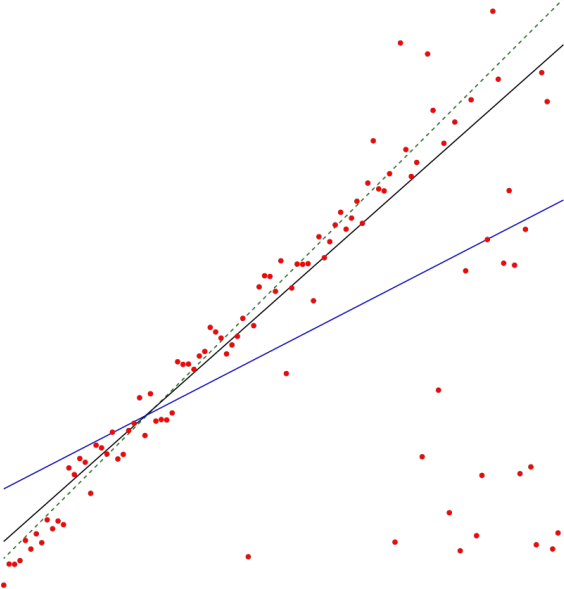
\includegraphics[width=0.6\linewidth]{linreg_error}
    \caption{Искажение результатов линейной регрессии небольшой долей выбросов}
    \label{img:linreg_errors}
\end{figure}

Причина такого поведения заключается в том, что квадрат отклонения быстро возрастает с ростом расстояния до моделируемой прямой, поэтому даже небольшое количество точек, полученных из другого распределения, приводят к большому штрафу для истинной прямой. Для улучшения результатов линейной регрессии следует заменить критерий \eqref{linreg_criterion} на другой, более устойчивый к выбросам.

\begin{definition}{$M$-оценка.}
    \textbf{$M$-оценкой} называется любая статистическая оценка, которая находится как решение уравнения следующего вида:
    \begin{equation}
    \label{m_est}
        \hat{\theta} = \arg\min_{\theta} \sum_{i=1}^{n} \rho\left( \eps(\theta, x_i) \right).
    \end{equation}
\end{definition}

В случае линейной регрессии функция $\eps$ вычисляет расстояние от точки до прямой, заданной параметрами $\theta$, а $\rho$ является штрафной функцией. Для того, чтобы модель получилась устойчивой к выбросам, нужно, чтобы $\rho\left( t \right)$ сравнительно быстро возрастала в окрестности нуля, после чего возрастание замедлялось бы.

Предположим, что мы выбрали функцию $\rho(t)$ и хотим научиться минимизировать ее.
Непосредственный перебор всех возможных параметров по некоторой дискретной равномерной сетке обладает высокой сложностью ($O\left( n_\rho n_\theta n \right)$).
Однако его можно ускорить при помощи преобразования Радона.
Необходимо найти такое преобразование изображения, чтобы сумма результата по прямой была равна значению функции потерь для этой прямой с точностью до знака.
После этого оптимальные параметры $\hat\theta$ можно будет найти следующим образом:
\begin{equation}
\label{m_est_radon}
    \hat\theta = \arg\max_{\theta} \left[ \mathcal{R} \left( K_{\rho}\left( \left\| \vec x \right\| \right) * I\left( \vec x \right) \right) \right]\left( \theta \right),
\end{equation}
где $I\left( \vec x \right) = \sum_{i=1}^n \delta\left( \vec x - \vec x_i \right)$ -- непрерывное изображение, соответствующее оцениваемому набору точек, $K_{\rho}\left( \left\| \vec x \right\| \right)$ -- некоторое центрально-симметричное ядро, которое нужно найти.
В соответствии в правилами свертки $K_{\rho}\left( \left\| \vec x \right\| \right) * I\left( \vec x \right) = \sum_{i=1}^n K_\rho\left( \left\| \vec x - \vec x_i \right\| \right)$.

Поскольку преобразование Радона линейно, достаточно рассмотреть случай, когда в наборе всего одна точка.
Для удобства предположим, что эта точка расположена в начале координат.
Сравнивая выражения \eqref{m_est}, \eqref{m_est_radon}, понимаем, что интеграл по прямой должен быть равен минус расстоянию от единственной точки до рассматриваемой прямой: $\left[ \mathcal{R}f \right]\left( \theta_0 \right) = -\rho\left( \theta_0 \right)$.
% минус -- потому что искать на Хаф-образе минимум, а не максимум, вероятно, религия не позволяет.

Пусть прямая задана таким образом, что ее точки задаются следующими уравнениями ($l$ -- натуральный параметр на прямой):
\begin{equation*}
    \begin{cases}
        x_1(\theta, l) = -l \sin\theta_1 + \theta_0 \cos\theta_1,\\
        x_2(\theta, l) =  l \cos\theta_1 + \theta_0 \sin\theta_1.
    \end{cases}
\end{equation*}

Так как мы рассматриваем центрально-симметричные ядра, то преобразование Радона от ядра $f\left( \vec x\left( \theta, l \right) \right) =: F\left( \sqrt{x_1^2 + x_2^2} \right) = F\left( \sqrt{l^2 + \theta_0^2} \right)$ сводится к преобразованию Абеля:
\begin{equation*}
    \left[ \mathcal{R}f \right]\left( \theta_0 \right) =
    \int_{\mathbb{R}} F\left( \sqrt{l^2 + \theta_0^2} \right) dl =
    \int_{|\theta_0|}^{+\infty} \frac{F(r)r}{\sqrt{r^2 - \theta_0^2}} dr.
\end{equation*}

К счастью, Абель также нашел обратное преобразование, позволяющее находить функцию $F(r)$ в зависимости от желаемых значений интеграла (при условии, что она убывает достаточно быстро):
\begin{equation*}
    F(r) =
    -\frac{1}{\pi} \int_r^\infty \frac{\left[ \mathcal{R}f \right]'\left( \theta_0 \right)}{\sqrt{\theta_0^2 - r^2}}d\theta_0 =
    +\frac{1}{\pi} \int_r^\infty \frac{\rho'\left( \theta_0 \right)}{\sqrt{\theta_0^2 - r^2}}d\theta_0.
\end{equation*}

Таким образом, для любой заданной функции $\rho$ можно найти соответствующее ядро. Итоговый алгоритм записывается следующим образом:
\begin{itemize}
\item
    Дискретизовать изображение $I\left( \vec x \right)$ в двумерную гистограмму.
\item
    Свернуть гистограмму с дискретизованным ядром, найденным при помощи обратного преобразования Абеля для желаемой целевой функции.
\item
    Вычислить быстрое преобразование Хафа.
\item
    Найти максимум в пространстве Хафа и вернуть параметры прямой, соответствующей этому максимуму.
\end{itemize}

Сложность алгоритма составляет $\Theta\left( N + w^2 n^2 + n^2 \log n \right)$, где $N$ -- количество точек, $n$ -- линейный размер квдаратной гистограммы, $w$ -- линейный размер используемого ядра.
